\documentclass[12pt, letterpaper]{article}
\usepackage[utf8]{inputenc}
\usepackage[italian]{babel}
\usepackage[T1]{fontenc}
\usepackage{graphicx}
\graphicspath{}

\title{Progetto corso di Progetto Automatico di Sistemi Digitali}
\author{Filippo Landi}

\begin{document}
\maketitle

\begin{abstract}
Il mio progetto per il corso di Progetto Automatico di Sistemi Digitali consiste nello studio statistico di alcuni possibili difetti in un circuito di tipo "multiply and accumulate" o "mac" in breve.
\end{abstract}

\section{Introduzione al progetto}

Per il progetto viene usato "HOPE", un software di Electronic Design Automation (EDA) sviluppato dalla università VirginiaTech: è un simulatore di guasto per circuiti digitali sequenziali e legge i circuiti in una descrizione (netlist) in formato ".bench".

La parte operativa di descrizione del circuito nel formato .bench e i calcoli statistici sui guasti saranno svolti per semplicità con degli script scritti in Python.  

\section{Circuito multiply and accumulate}

Come prima cosa mi è stato richiesto di realizzare un circuito multiply and accumulate (mac) a 8 bit.
Ho ricevuto un documento dal professore che illustra gli schemi di un circuito di questo tipo a 4 bit, più alcuni commenti utili: vista la dimensione riporto questa documentazione nella pagina seguente.
\newpage
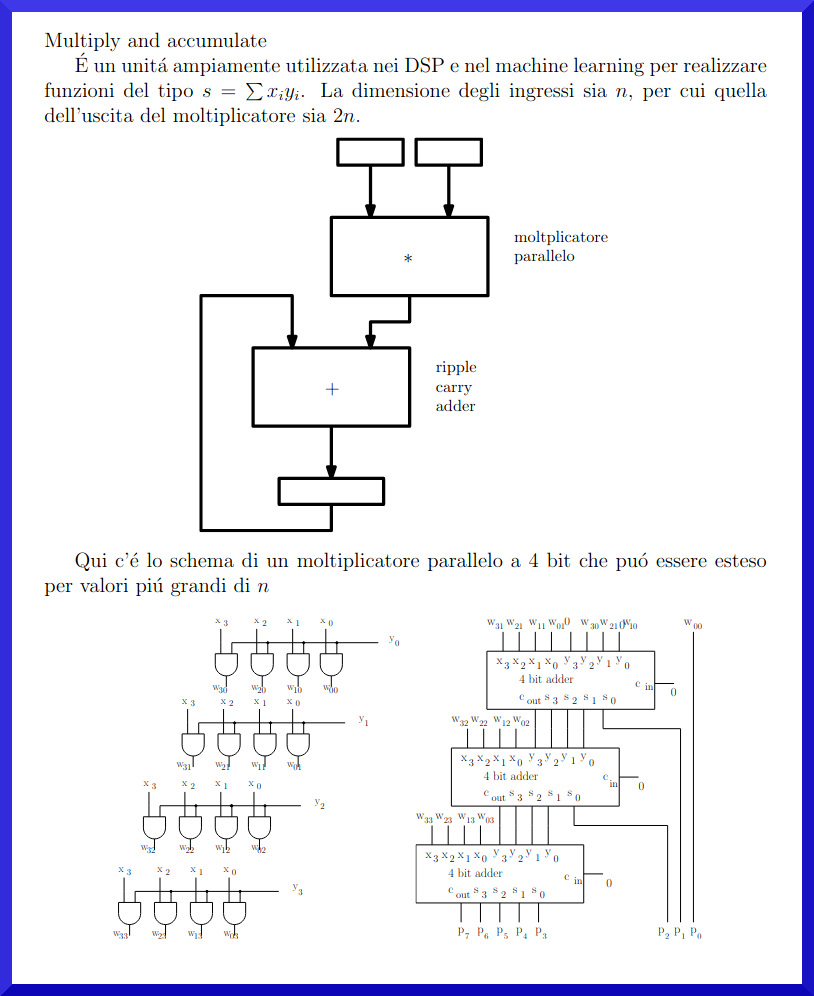
\includegraphics[width=\textwidth]{mac.png}
\newpage

\subsection{Moltiplicatore}
La struttura del moltiplicatore è ben illustrata nella documentazione:

\begin{itemize}
  \item Ogni segnale X è messo in ingresso con ogni Y, generando i segnali W.
  \item I segnali W vengono usati da ripple carry adder strutturati su più livelli: si può notare che il numero di livelli è n-1 in quanto al primo livello vengono usati WX1 e WX0, poi i rimanenti WXY nei livelli successivi.
\end{itemize}

\subsection{Ripple Carry Adder}

I ripple carry adder nella precedente documentazione erano illustrati la livello register transfer level (RTL) per ovvie ragioni di chiarezza.
Per l'implementazione del circuito ci serve vedere come sono fatti a livello di porte logiche.  
I ripple carry adder sono circuiti formati da una serie di adder in cascata:
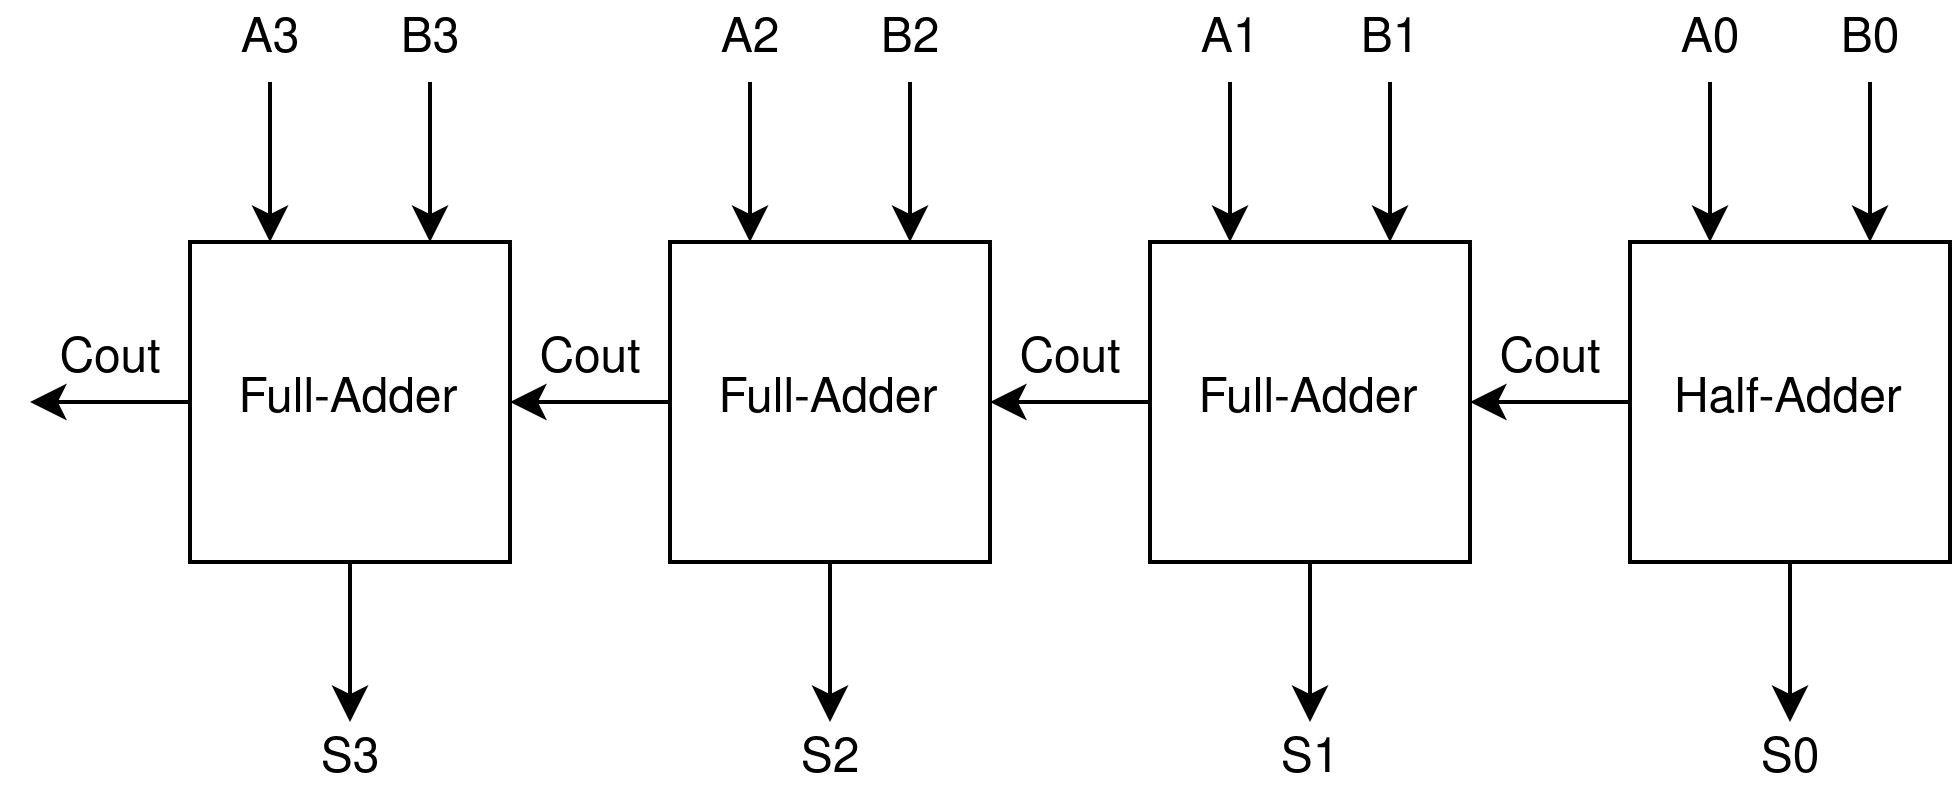
\includegraphics[width=\textwidth]{ripple_carry_adder}

Questo è lo schema che uso del half-adder:
\begin{center}

\includegraphics{half_adder}
\end{center}

Questo è lo schema che uso del full-adder:
\begin{center}
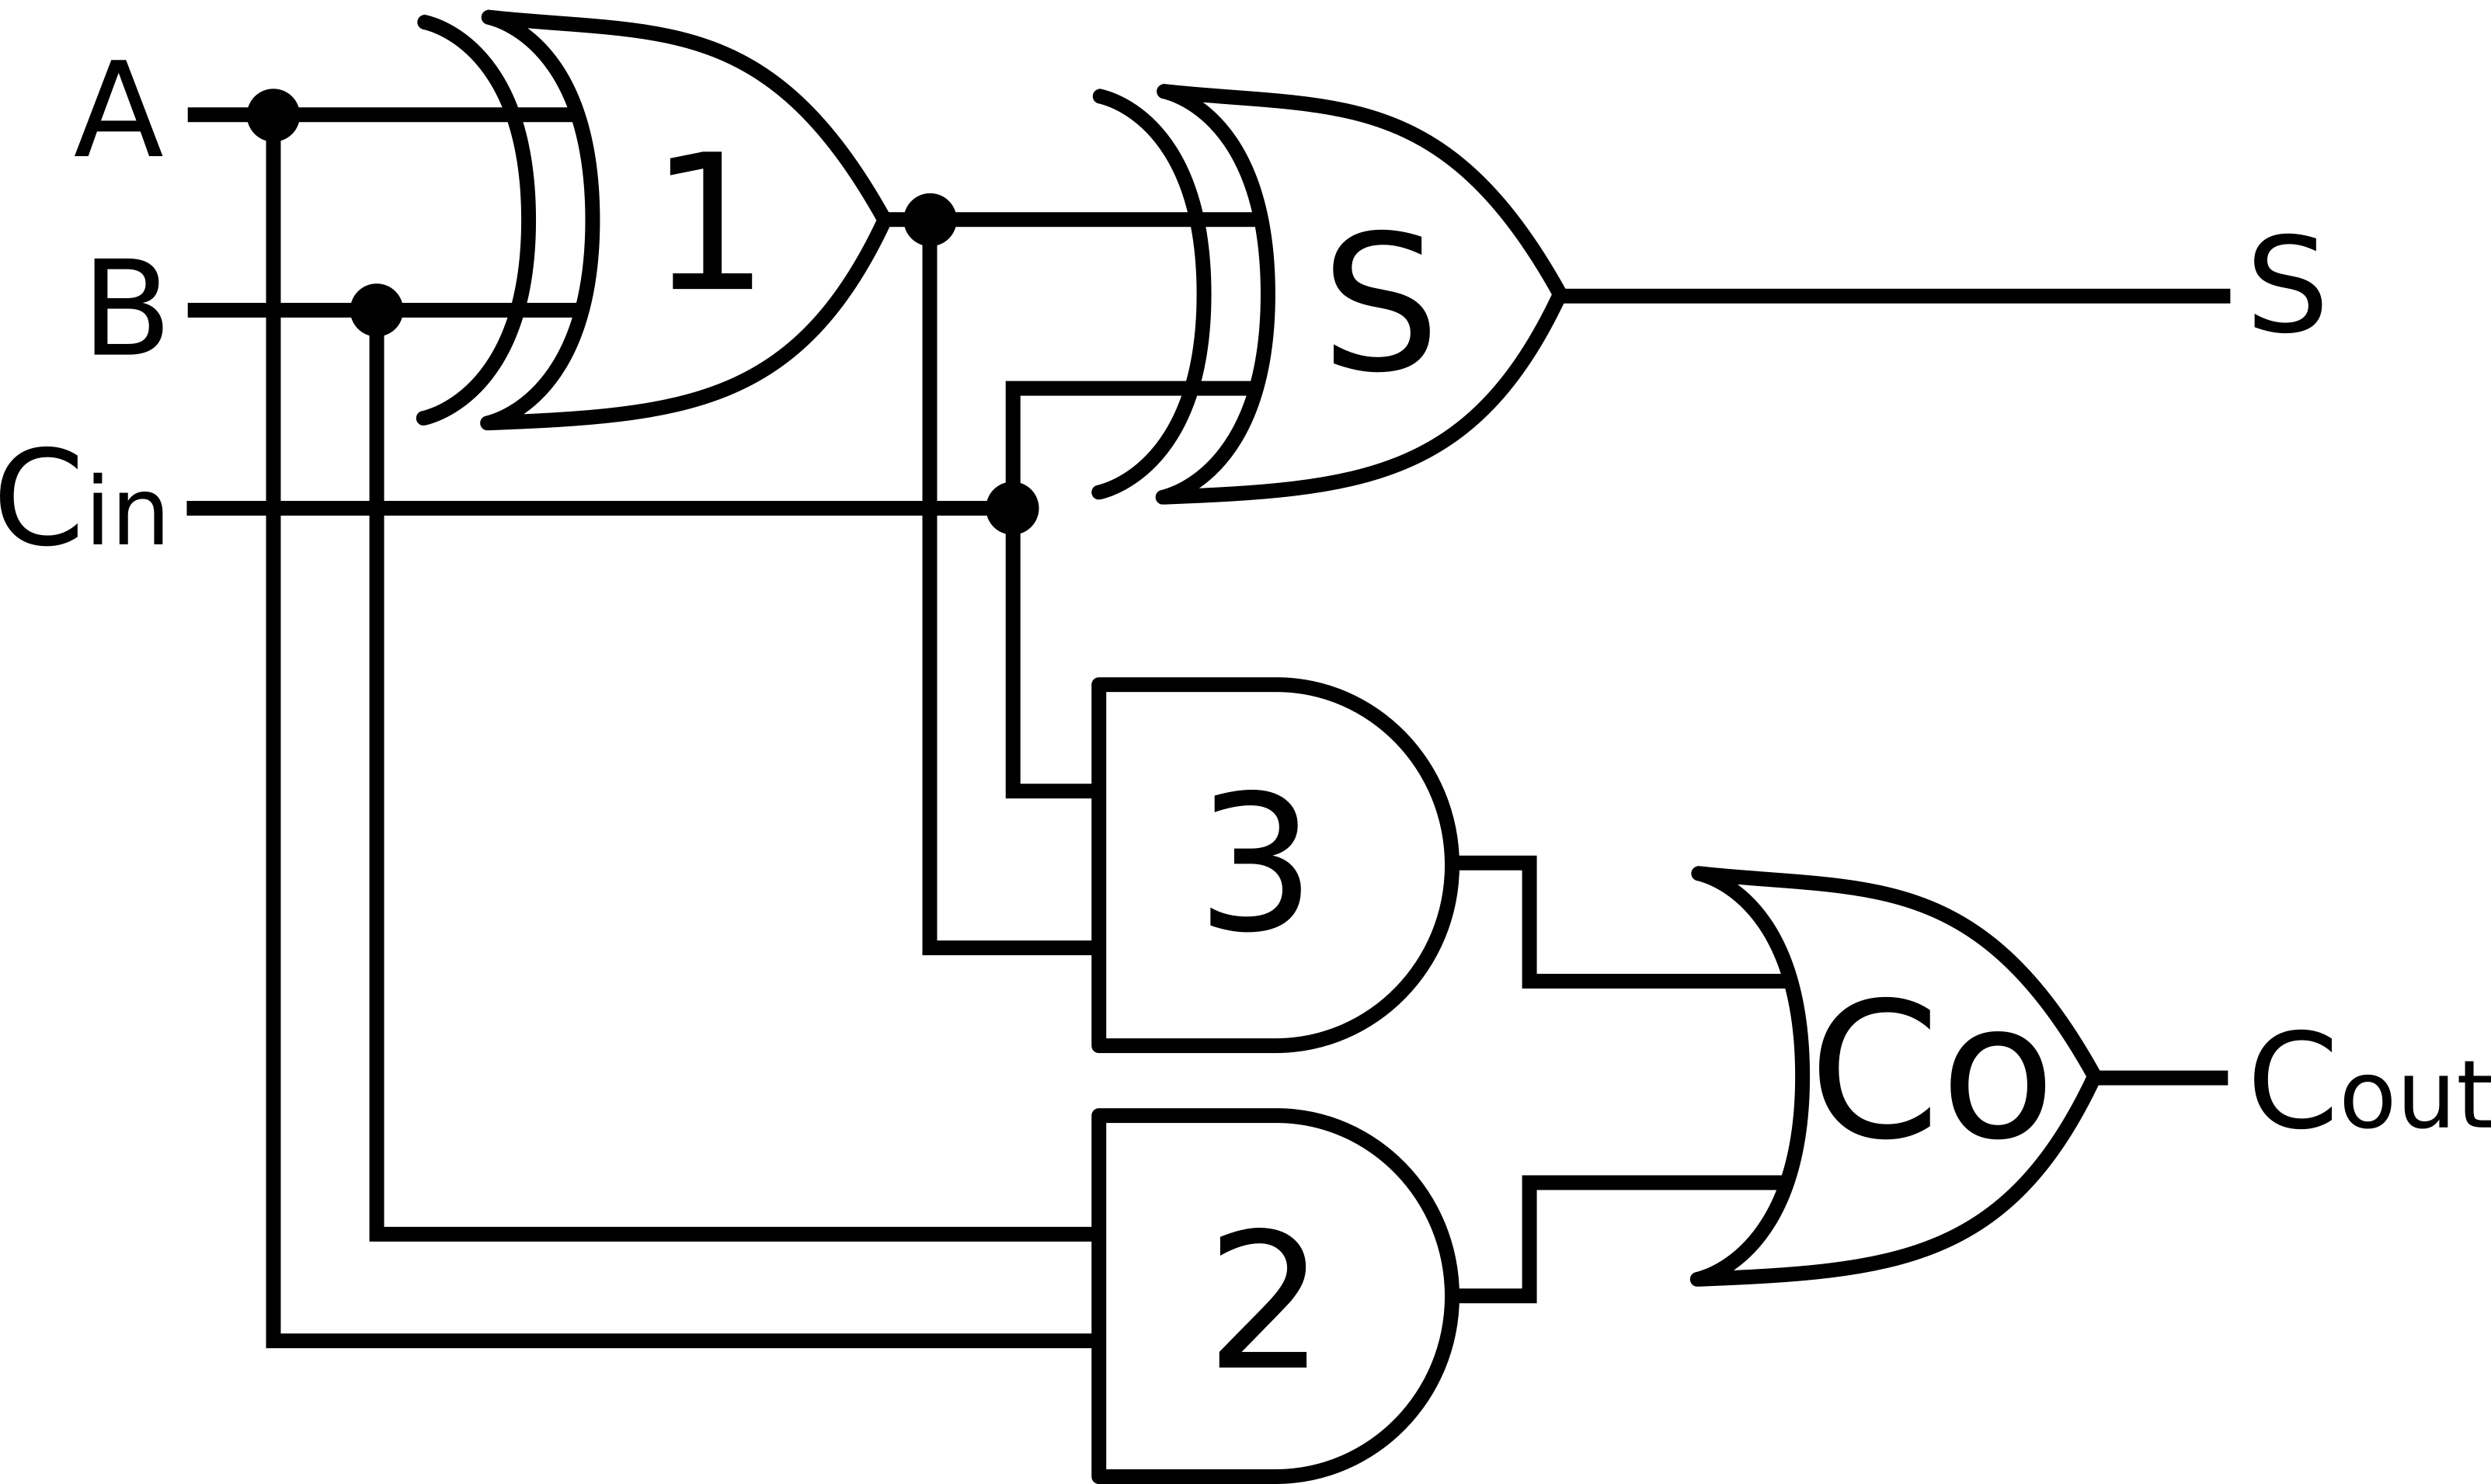
\includegraphics[width=8cm]{full_adder}
\end{center}

Opportunamente collegando i vari segnali e circuiti quindi si ottiene un ripple carry adder.
Abbiamo dei ripple carry adder sia per la cascata di ripple carry adder per il moltiplicatore che per la seconda parte del circuito che è un sommatore (di ingressi 2n).

\subsection{Sommatore}
Come già detto si sfruttano gli stessi schemi riportati prima, solo che qui il ripple carry adder è di dimensione doppia rispetto a quelli del moltiplicatore.
Un ingresso è dato dall'uscita del moltiplicatore mentre l'altra è data dalle uscite stesse del sommatore retroazionate grazie a dei flip flop tipo D (circuito già integrato in HOPE).

\section{Realizzazione del circuito in Python}

La stesura manuale del circuito a 8 bit non mi sembrava un approccio furbo al problema poiché è facile commettere errori sia (banalmente) di battitura sia dovuti ad una scarsa comprensione dell'architettura del circuito.

Il mio approccio quindi è stato quella di scrivere uno script in Python che descrivesse e collegasse le varie parti del circuito.  

In partenza ho scritto alcuni circuiti di prova, che trovate nella cartella "circuti\_prova", non sono fondamentali per il progetto però credo che possano aiutare alla comprensione della metodologia usata.

Questo approccio mi ha permesso di arrivare ad uno script che permette di generare il circuito con una dimensione arbitraria degli ingressi da passare come argomento: ad esempio per generare un mac 4 bit si può scrivere da terminale questo comando Python: "python3 mac\_generator 4".

Al momento sul mio computer ho installato Python 3.8.10, quindi credo che una qualsiasi versione di Python 3.8 non dovrebbe dare problemi col mio codice.

Il codice è ampiamente commentato e credo che i commenti siano sufficienti a capire il funzionamento per questo non riporto il codice in questa documentazione.

Riporto giusto qualche considerazione:
\begin{itemize}
  \item Serve una conoscenza base del linguaggio Python per capire a pieno il codice.
  \item I nomi dei segnali sono come riportati negli schemi con l'aggiunta per differenziarli dell'indice del livello a cui appartengono: ad esempio l'S0 del primo livello di rca del moltiplicatore è ovviamente differente dall'S0 del secondo livello per questo nel codice sono definiti SL0D0 e SL1D0, con L che indica il livello D il peso del bit.
  \item L'idea principale è quella di usare cicli for variando opportunamente gli indici dei segnali, gli schemi dei circuiti si ripetono spesso tranne per qualche eccezione riportata nei commenti del codice.
  \item Tutti i segnali di carry sono definiti come carry out (Co nel codice), di fatto i carry in sono il carry out dell'adder precedente quindi coincidono.
\end{itemize}

\end{document}


